\documentclass[conference]{IEEEtran}
\usepackage{parskip}
\usepackage{fdsymbol}
\usepackage{microtype}
% \usepackage{natbib}
\usepackage[dvipsnames]{xcolor}
\usepackage[draft]{graphicx}
\usepackage{url}
\usepackage{booktabs}
\usepackage{array}
\usepackage{tabularx}

\usepackage{hyperref}
\usepackage[noabbrev,nameinlink,capitalize]{cleveref}

\graphicspath{{.}{./pictures}{./figures}}

\bibliographystyle{IEEEtran}

\title{Knowledge Grounding in Large Language Models: \\ An Empirical Study}

\newcommand{\spade}{$\phantom{}^\spadesuit$}
\author{%
	Martin~Fixman\spade{}, Tillman~Weyde\spade{}, Chenxi~Whitehouse\spade{}, Pranava~Madhyastha\spade{} \\
	$\phantom{}^\spadesuit{}$ City St.\ George's, University of London%
}

\newcommand{\Parametric}{\textbf{\textcolor{ForestGreen}{Parametric}}}
\newcommand{\Contextual}{\textbf{\textcolor{Maroon}{Contextual}}}
\newcommand{\Other}{\textbf{\textcolor{MidnightBlue}{Other}}}

\newcommand{\smallflan}{\texttt{flan-t5-xl}}
\newcommand{\bigflan}{\texttt{flan-t5-xxl}}
\newcommand{\smallllama}{\texttt{Meta-Llama-3.1-8B-Instruct}}
\newcommand{\bigllama}{\texttt{Meta-Llama-3.1-70B-Instruct}}

\newcommand{\llamaparbox}{\parbox{65pt}{\centering\ttfamily Meta-Llama-3.1 \\ -8B-Instruct}}
\newcommand{\bigllamaparbox}{\parbox{65pt}{\centering\ttfamily Meta-Llama-3.1 \\ -70B-Instruct}}

\newcommand{\todo}[1]{\textcolor{red}{\sffamily \textbf{TODO}: #1}}

\begin{document}

\maketitle{}

\begin{abstract}
	\begin{abstract}

In recent years large language models have exploded in quality and prevalence, and they have become crucial for work in a wide range of areas.
However, their tendency to produce hallucinations presents a critical challenge in contexts where precision and correctness are crucial.

Retrieval-Augmented Generation (RAG), which leverages external information to provide more accurate and contextually appropriate responses, has been proposed as a solution to this problem.
However, this solution is far from perfect as it's unclear when a large language model will choose to generate answers using the context provided by RAG over the knowledge in its parametric memory.

This thesis explores the \emph{Knowledge Grounding} of various large language models.
In particular, it attempts to answer a research question: \textbf{How does a large language model respond to questions when context  information contradicts or supports its inherent parametric knowledge?}

To investigate this, we develop a diverse dataset comprising questions on various topics and using diverse data.
We use this dataset to construct queries with counter-parametric context, i.e. the context information contradicts the answer given by the model without context, and parametric context. We test models of different architectures and sizes to find out which type of answer they choose.
We also analyse the \emph{perplexity} of these answers to give us an indication on certainty of the model in its answer, and observe differences in the perplexity between answers that agree or disagree with the context information. 

Our findings suggest that smaller models and models that encode the entire input sequence into an internal representation before outputting an answer might produce more answers sourced from the RAG-provided context, therefore avoiding hallucinations.
In particular, the smaller models \texttt{Meta-Llama-3.1-8B} and \texttt{Flan-T5-XL} tend to have better knowledge grounding and fewer hallucinations than their larger versions, while encoder-decoder Seq2Seq models tend to outperform Decoder-only models.
As an additional analysis we investigate methods for determining whether a given response originates from the RAG context or the model's internal memory from the query's resulting perplexity.
This might be used to develop methods to prevent hallucinations in large language models that use RAG indexing.

% This thesis forms the foundational part of a broader project aimed at publishing a comprehensive study on knowledge grounding in retrieval-augmented language models, as outlined in the unpublished preprint ``Knowledge Grounding in Retrieval-Augmented LMs: An Empirical Study'' \citep{knowledge_grounding_retrieval_augmented}.
% We build on existing literature, incorporating the use of counterparametric context in queries, to advance our understanding of this phenomenon.

\end{abstract}

\end{abstract}

\section{Introduction and Objectives}
% This structure is copied from Nikolai Manchev.

\subsection{Problem Background}

In recent years, Large Language Models (LLMs) have become ubiquitous in solving general problems across a wide range of tasks, from text generation to question answering and logic problems.
However, recent research suggests that using these models alone might not be the most effective way to solve problems that are not directly related to text generation \citep{treeofthoughts}.

One approach to improving the performance on knowledge problems for LLMs is Retrieval-Augmented Generation (RAG) \citep{rag}. RAG involves retrieving relevant context related to a query and incorporating it into the model's input, enhancing the model's ability to generate accurate and contextually appropriate responses.

As RAG-enhanced systems become more widespread, studies on the performance of different retrieval systems and their interaction with LLMs have become crucial.
Many explore the performance of these downstream tasks depending on both the retriever and the generator \citep{can_rag_models_reason,gpt3}, examining whether the knowledge is \textit{grounded} in the context.
Retrieval-Augmented models, such as \textsc{Atlas} \citep{atlas_foundational} and \textsc{Retro} \citep{retro}, use this approach to fine-tune a model on both a large body of knowledge and an existing index for context retrieval.

This project aims to understand the performance of various large language models with added context by measuring their \textit{knowledge grounding} on a dataset consisting of a large variety of questions across a wide range of topics.
We follow the approach by \citeauthor{factual_recall} of running queries with counterparametric context to understand whether a particular answer originates from the model's inherent knowledge (i.e., its training data) or from the provided context (i.e., the context retrieved by RAG).

This thesis builds on this knowledge and improve our understanding of how different LLMs interact with the given context in the problem of question answering.
Specifically, we investigate whether these interactions vary depending on the type of question being answered, contributing to a more nuanced understanding of LLM performance in diverse knowledge domains.

\subsection{Research Question}

How do we know what large language models really know?
This thesis attempts to answer this question by asking a different but related question:

\textbf{How does a large language model respond when given information that contradicts its inherent knowledge, and why?}

The rest of this section gives an overview of the steps we take to answer this question.

\subsection{Research Objectives}
\label{introduction_research_objectives}

This thesis is structured around three different sub-objectives to deepen our understanding knowledge grounding in large language models.

% We propose the creation of a novel dataset of questions designed for testing LLMs' ability to distinguish between parametric and contextual knowledge.
% This dataset is used to investigate the factors influencing an LLM's choice of answer, and hypothesise that we can use perplexity scores as a predictor of where a particular answer originates.

\begin{description}[style=nextline,labelindent=10pt,itemindent=25pt]
	\item[1. Creating a representative dataset of questions.]
		This is necessary as existing Q\&A datasets are not suitable for our objectives.
	\item[2. Building an experimental framework to understand the source of an LLM's answer.]
		This will give us information about which models prefers which type of answers, whether it depends on the question asked, and more.
	\item[3. Enhancing the framework to understand the reasoning behind each answer]
		We use the perplexity of a model's response on both answers to understand \textit{why} a certain answer was chosen.
\end{description}

\subsection{Overview of Methods}

\subsubsection{Creating a representative dataset of questions}
\label{questions_objective}

We require a dataset of questions that's useful for answering our research question.
This dataset should allow us to understand the responses of the models to know whether they came from the model's parametric memory or from the RAG context, and should be reasonably representative of the world to prevent biases.

In particular, the questions should allow us to easily create counterparametric answers to later add as context to our queries.
We follow the example of \citeauthor{factual_recall} on creating questions that can be easily answered with short responses, and later using these answers to create counterparametric context.

We also enhance this work by adding a much larger set of questions of a variety of topics.

\subsubsection{Building an experimental framework to understand the source of an LLM's answer}
\label{intro_models_numbers}

Currently, little is understood about the factors and mechanisms that control whether an LLM will generate text respecting either the context or the memorised information.

Previous research found out that, when the context of a query contradicts the ground knowledge of a model, the final answer depends on the size and architecture of the model used \citep{factual_recall}.

This thesis extends this research by testing the representative set of questions and counterfactuals described in the previous section with both Seq2Seq and Decoder-only models of various sizes.
We also research the cases when the answer doesn't correspond to either the parametric or contextual knowledge, and why the model chooses a third type of answer when adding counterfactual context.

% This thesis also gathers insights from answering this question on different categories and patterns of questions to find out if this depends on what is being asked.

\subsubsection{Enhancing the framework to understand the reasoning behind each answer}

\Citeauthor{factual_recall} showed that there is a correlation between the probability of a large language model choosing a parametric answer over a counterfactual contextual answer and the amount of times this answer appears in the ground truth data of the model.
This gives us clues on whether the result of a query came from parametric or contextual knowledge if we have access to this ground truth, as is the case in models like Pythia \citep{pythia}.

Unfortunately, most so-called open-source large language models do not give us access to the source data being used to train it and therefore do not allow this kind of analysis.

The \textbf{perplexity} score of answer gives a measure of how ``certain'' a large language model is of its answer \citep{how_can_we_know}.
We hypothesise that we can use this metric to serve as a reliable indicator of whether a particular answer was memorised by the LLM or was derived from the provided context.


\section{Related Work}
\label{related_work}

% Putting this input here so LaTeX can place it in the right page.
\begin{table*}[t]
	\centering
	\small

	\newcommand{\qtbox}[1]{\parbox{190pt}{#1}}
	\newcommand{\qwbox}[2]{\setlength{\fboxsep}{0pt}\fbox{\colorbox{#1}{\strut \rule{0pt}{8pt}\hspace{1pt}#2\hspace{1pt}}}}
	\newcommand{\qwtext}[2]{\textbf{\color{#1}{#2}}}

	\newcommand{\qwabox}[1]{\qwbox{BurntOrange}{#1}}
	\newcommand{\qwatext}[1]{\qwtext{BurntOrange}{#1}}
	\newcommand{\qwbbox}[1]{\qwbox{ForestGreen}{#1}}
	\newcommand{\qwbtext}[1]{\qwtext{ForestGreen}{#1}}
	\newcommand{\qwcbox}[1]{\qwbox{Thistle}{#1}}
	\newcommand{\qwctext}[1]{\qwtext{Thistle}{#1}}
	\newcommand{\qwdbox}[1]{\qwbox{SkyBlue}{#1}}
	\newcommand{\qwdtext}[1]{\qwtext{SkyBlue}{#1}}
	\newcommand{\qwebox}[1]{\qwbox{Melon}{#1}}
	\newcommand{\qwetext}[1]{\qwtext{Melon}{#1}}

	\newcommand{\qwfbox}[1]{\qwbox{Dandelion}{#1}}
	\newcommand{\qwftext}[1]{\qwtext{Dandelion}{#1}}

	\begin{tabular}{l @{\hspace{-15pt}} r @{\hspace{7pt}} c @{\hspace{50pt}} c @{\hspace{5pt}} l}
		\toprule
			\bfseries Initial Query & \bfseries Parametric Answer && & \bfseries Query with Counterparametric Context \\
		\midrule
			\qtbox{Q: What country is \qwabox{Cairo} in? \\ A: \qwabox{Cairo} is in} & \qwatext{Egypt} & \tikzmark{egyptAnswer} & \tikzmark{usaCtx} & \qtbox{[\qwabox{Cairo} is in \qwbtext{the United States}] \\ Q: What country is \qwabox{Cairo} in? \\ A: \qwabox{Cairo} is in} \\[20pt]
			\qtbox{Q: What country is \qwbbox{New York} in? \\ A: \qwbbox{New York} is in} & \qwbtext{the United States} & \tikzmark{usaAnswer} & \tikzmark{egyptCtx} & \qtbox{[\qwbbox{New York} is in \qwatext{Egypt}] \\ Q: What country is \qwbbox{New York} in? \\ A: \qwbbox{New York} is in} \\[20pt]
			\qtbox{Q: What country is \qwcbox{Bangkok} in? \\ A: \qwcbox{Bangkok} is in} & \qwctext{Thailand} & \tikzmark{thailandAnswer} & \tikzmark{usaCtx2} & \qtbox{[\qwcbox{Bangkok} is in \qwbtext{the United States}] \\ Q: What country is \qwcbox{Bangkok} in? \\ A: \qwcbox{Bangkok} is in} \\[20pt]
			\qtbox{Q: What country is \qwfbox{San Francisco} in? \\ A: \qwfbox{San Francisco} is in} & \qwftext{the United States} & & \tikzmark{thailandCtx} & \qtbox{[\qwfbox{San Francisco} is in \qwctext{Thailand}] \\ Q: What country is \qwfbox{San Francisco} in? \\ A: \qwfbox{San Francisco} is in} \\[20pt]
			\qtbox{Q: What is the date of birth of \qwdbox{Che Guevara}? \\ A: The date of birth of \qwdbox{Che Guevara} is} & \qwdtext{June 14, 1928} & \tikzmark{guevaraAnswer} & \tikzmark{diocletianCtx} & \qtbox{[\qwdbox{Che Guevara} was born in \qwetext{245 CE}] \\ Q: What is the date of birth of \qwdbox{Che Guevara}? \\ A: The date of birth of \qwdbox{Che Guevara} is} \\[20pt]
			\qtbox{Q: What is the date of birth of \qwebox{Emperor Diocletian}? \\ A: The date of birth of \qwebox{Emperor Diocletian} is} & \qwetext{245 CE} & \tikzmark{diocletianAnswer} & \tikzmark{guevaraCtx} & \qtbox{[\qwebox{Emperor Diocletian} was born in \qwdtext{June 14, 1928}] \\ Q: What is the date of birth of \qwebox{Emperor Diocletian}? \\ A: The date of birth of \qwebox{Emperor Diocletian} is} \\[10pt]
		\bottomrule \addlinespace[4pt]
	\end{tabular}

	\begin{tikzpicture}[remember picture, overlay, ->, >=stealth, thick]
		\draw (pic cs:egyptAnswer) +(0pt, 2pt) to (pic cs:egyptCtx);
		\draw (pic cs:usaAnswer) +(0pt,  4pt)  to (pic cs:usaCtx);
		\draw (pic cs:usaAnswer) +(0pt, 0pt) to (pic cs:usaCtx2);
		\draw (pic cs:guevaraAnswer) +(0pt, 2pt) to (pic cs:guevaraCtx);
		\draw (pic cs:diocletianAnswer) +(0pt, 2pt) to (pic cs:diocletianCtx);
		\draw (pic cs:thailandAnswer) +(0pt, 2pt) to (pic cs:thailandCtx);
	\end{tikzpicture}

	\caption{Example of counterparametric context being added to a query on cities. Arrows represent the random shuffling of parametric answers to add to the counterparametric context of a new query with the same base question. We ensure parametric answers aren't shuffled into the context or another question with the same answer, as in the cases with New York and San Francisco.}
	\label{counterparametric_example}
\end{table*}


\textbf{Hallucinations in Large Language Models}
The success of machine learning models based on transformer architecture~\cite{attention_is_all_you_need} has enabled the development of large-scale language models such as GPT-3~\cite{gpt3} and Llama~\cite{llama}.
Despite their advancements, factual reliability remains a significant issue.

Recent studies such as Jiang et al.~\cite{how_can_we_know} highlighted the prevalence of hallucinations across tasks, particularly in factual contexts.
Other studies, such as Ghader et al.~\cite{can_rag_models_reason}, emphasize the challenge of ensuring accuracy in generated text.

These concerns have prompted a wave of research focused on evaluating and mitigating hallucinations.

\textbf{Parametric and Contextual Knowledge} 
The distinction between parametric knowledge (stored in the model's weights) and contextual knowledge (provided in the input) has been a focal point of several studies~\cite{knowledge}.

Yu et al.~\cite{factual_recall} investigated how factors like training data, architecture, and fine-tuning affect the interplay between these two knowledge sources.
Similarly, Tuan et al.\cite{when_context_leads} explored how language models balance parametric and contextual knowledge when answering open-ended questions by systematically varying context sizes to analyze when models prioritize provided context over their internal knowledge.
Their findings suggest that while LLMs are capable of incorporating contextual information, they often default to their parametric memory when faced with ambiguous or conflicting inputs.
% Their work suggests that encoder-decoder models, such as T5~\cite{t5,flant5}, are generally more effective at using input context compared to decoder-only models, which often struggle to override their internal knowledge.

Building on this, Cheng et al.~\cite{understanding_the_interplay} systematically explores how parametric and contextual knowledge interact, identifying scenarios where contextual knowledge can degrade performance, even when complementary.

Through this lens, our work contributes to the understanding of how model architecture, and size shape knowledge grounding in large language models.

\textbf{Knowledge Probing Datasets}: Prior work has developed datasets to evaluate LLMs' factual knowledge, including Natural Questions~\cite{natural_questions} and Countries' Capitals~\cite{factual_recall}. However, these datasets are not designed to analyze how models arbitrate between their parametric knowledge and contradictory contextual information, which is the focus of our study.

In particular, while the Natural Questions dataset offers a wide range of questions, its lack of systematic categorization hinders counterparametric experiments.
The Countries' Capitals dataset, while well-suited for counterparametric evaluation, is limited in scope.

\textbf{Retrieval-Augmented Generation} (RAG)~\cite{rag} attempts to improve factual accuracy by integrating external knowledge during inference.
However RAG does not always ensure that language models prioritize the retrieved evidence over their parametric knowledge as evidenced by the research by Yu et al.~\cite{factual_recall} and Hsia et al.~\cite{ragged}: even when presented with contradictory context, models often rely on their parametric memory.
Our study builds on these observations, examining this behavior across various model architectures and sizes.


\section{Experimental Setup}


\section{Results}
\label{results_section}

\subsection{Experimental Setup}

The code for running the framework is included along with the questions used in this Github repository: \texttt{\url{https://github.com/mfixman/knowledge-grounding-in-llms}}.
The repository contains instructions on how to use it with different datasets and LLMs.

The experiments in this research were run on a server with 48 Intel(R) Xeon(R) CPU 3GHz CPUs, 376GB of RAM, and 2 NVIDIA A100 GPUs with 80GB of VRAM each. 
%that was kindly provided to Artificial Intelligence MSc students in at City St George's, University of London.

\subsection{Experimental Results}

\begin{table}[t]
	\caption{Amount of answers of each category when running our dataset on each of the four models.}
	\label{total_table}
	\centering
	\footnotesize
	\begin{tabular}{l r r r}
		\toprule
			\bfseries Model & \Pc{} & \Cc{} & \Oc{} \\
		\midrule
			\smallflan{}  & 248 & 4284 & 228 \\
			\bigflan{} & 242 & 4304 & 214 \\
		\midrule
			\smallllama{} & 745 & 3662 & 353 \\
			\bigllama{} & 1070 & 3303 & 387 \\
		\bottomrule \addlinespace[4pt]
	\end{tabular}
\end{table}

\begin{figure}[t]
	\centering
	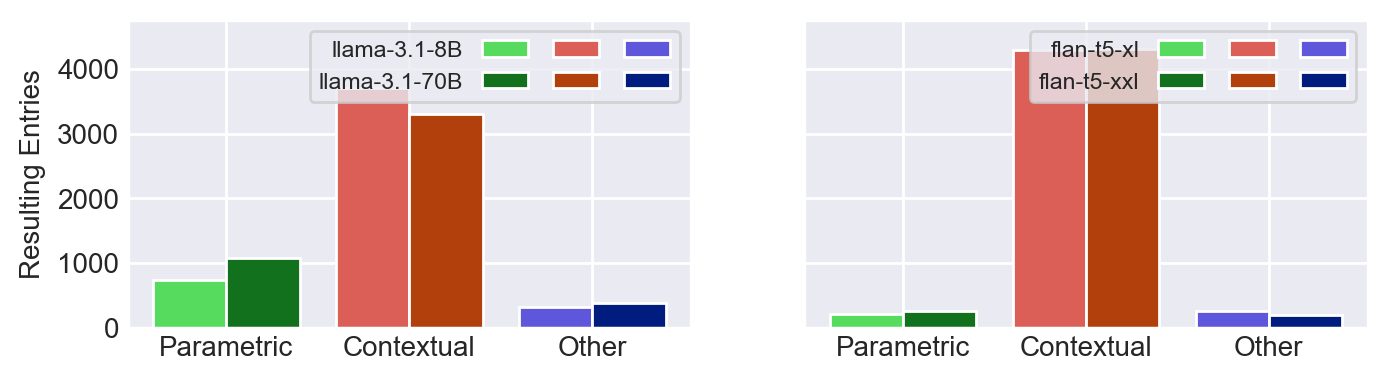
\includegraphics[width=\columnwidth]{both_amount.png}
	\caption{Amount of each answers of each category when running a context with counterparametric information for encoder-decoder and Decoder-only models of different sizes.}
	\label{total_plot}
\end{figure}

\begin{table*}[t]
	\caption{Results for each model tested on queries with counterparametric context in each one of the 10 given categories.}
	\label{cats_table}
	\centering
	\footnotesize
	\begin{tabular}{>{\bfseries}l | r r r | r r r | r r r | r r r}
		\toprule
			& \multicolumn{3}{c|}{\smallflan{}} & \multicolumn{3}{c|}{\bigflan{}} & \multicolumn{3}{c|}{\texttt{llama-8B}} & \multicolumn{3}{c}{\texttt{llama-70B}}  \\
			& \Pc{} & \Cc{} & \Oc{} & \Pc{} & \Cc{} & \Oc{} & \Pc{} & \Cc{} & \Oc{} & \Pc{} & \Cc{} & \Oc{}  \\
		\midrule
			Person           &  32 &  900 & 37 &  23 &  890 & 56 &  40 &  833 & 96 & 209 & 614 & 146 \\
			City             & 120 & 1030 & 40 &  78 & 1093 & 19 & 117 & 1007 & 66 & 166 & 966 &  58 \\
			Principle        &  13 &  164 &  8 &   9 &  168 &  8 &  44 &  118 & 23 &  44 & 117 &  24 \\
			Element          &   6 &  637 &  2 & 102 &  515 & 28 & 218 &  385 & 42 & 275 & 347 &  23 \\
			Book             &  26 &  488 & 25 &  18 &  457 & 64 & 135 &  344 & 60 & 154 & 318 &  67 \\
			Painting         &  26 &  446 & 56 &   4 &  498 & 26 &  47 &  458 & 23 &  49 & 445 &  34 \\
			Historical Event &  11 &  217 & 28 &   1 &  254 &  1 &  81 &  154 & 21 & 117 & 118 &  21 \\
			Building         &  14 &  174 & 10 &   0 &  189 &  9 &  27 &  163 &  8 &  31 & 159 &   8 \\
			Music      &   0 &  228 & 22 &   7 &  240 &  3 &  36 &  200 & 14 &  25 & 219 &   6 \\
		\bottomrule \addlinespace[4pt]
	\end{tabular}
\end{table*}

The results of running the queries with the questions created in \cref{dataset_creation} with added counterparametric context on each of the four models are shown in 
\Cref{total_table}. 
It shows the frequency of each type of answer for each one of the models,
i.e. the number of answers with a particular source for each one of the models when asking queries for all 4760 questions.

% Of the encoder-decoder models, \smallflan{} has $248$ answers from \Parametric{} knowledge ($5.21\%$), $4284$ answers from \Contextual{} knowledge ($90\%$), and $228$ answers from \Other{} source ($4.79\%$).
% \bigflan{} has a similar distribution of answers with $242$ \Parametric{} answers ($5.08\%$), $4304$ \Contextual{} answers ($90.42\%$), and $214$ \Other{} answers ($4.5\%$).

% The decoder-only models also have a majority of \Contextual{} answers, but have an otherwise different distribution with a smaller majority.
% \smallllama{} has $745$ answers from \Parametic{} knowledge ($15.65\%$), $3662$ answers from \Contextual{} knowledge ($76.93\%$), and $353$ answers from some \Other{} source ($7.42\%$).
% Unlike the previous architecture, the larger model \bigllama{} has a significantly different result with $1070$ \Parametric{} answers ($22.48\%$), $3303$ \Contextual{} answers ($69.39\%$), and $387$ \Other{} answers ($8.13\%$).
This information is also plotted in \cref{total_plot}, where the differences between %architectures and sizes
values can be visually appreciated.

\Cref{cats_table} contains the information separated by question category.
That is, for each model being tested with counterparametric data added to the context, how many questions in each category have answers from the \Parametric{} knowledge of the model, the \Contextual{} information in the query, and some \Other{} source.

The following sections discuss the reasons for the differences in distributions of the source of these answers along different models, and in the differences between different categories.


\section{Discussion}
\label{discussion}

\Cref{framework_results} presented results from generating the question dataset and running the framework to understand the role of knowledge grounding in a variety of models and their parametric knowledge in question-answering.
This section explains these results, and discusses what they mean for our research question.

\subsection{Model architecture and memorised knowledge}
\label{model_architecture_parametric}

\Cref{total_table,total_plot} show the total amount of \Parametric{}, \Contextual{}, and \Other{} answers from each model.
\Cref{cats_table} shows these results separated by category.

When taking into account model architecture, the results are clear: Seq2Seq models tend to answer questions from their contextual knowledge rather than from their inherent knowledge more often than Decoder-only models.
These results persist across different question categories and are consistent regardless of answer types and lengths

In the framework of question-answering when using RAG to fetch contextual data from an index, Seq2Seq models might tend to have fewer hallucinations that contradict this index than Decoder-only models.
We propose two hypotheses that could explain these differences.

\subsubsection{Inherent Advantages of the Encoder-Decoder Architecture}

Seq2Seq models such as \texttt{Flan-T5} are encoder-decoder models that process the entire context of the query in the encoder component before passing it to the decoder, which could increase the weight given to the context itself \cite{flant5}.

\subsubsection{Different training data and fine-tuning}

It's possible that these result doesn't come from the model architecture, but from the bias caused by their training methodology.

The \texttt{Flan-T5} models were trained on masked token generation and later fine-tuned on question-answering about passages \cite{flant5}.
This requires strong alignment between query and answer, which encourages the model to focus on the input context and makes it more likely to take the answer from the RAG-provided context.

Llama models were trained mainly on open-ended text generation, which relies more on parametric data.

It's possible that the deficiencies of knowledge grounding in Llama models might come simply to not being trained on related tasks.

\subsection{Model size and memorised knowledge}
\label{model_size_parametric}

\Cref{framework_results} also shows differences in how models of different sizes process information in queries with counterparametric context.

\subsubsection{Seq2Seq Models}

While the average results are very similar, which is likely due to the properties of Seq2Seq models discussed in \cref{model_architecture_parametric}, there seems to be a significantly lower amount of parametric answers in the larger Flan model for the categories of \emph{Element} and \emph{Historical Event}.
This is likely the case of the short questions answers: these categories have more questions that can be answered with answers that are 1- or 2-tokens long.

However, we can conjecture that overall the size of a Seq2Seq model has little overall impact on its knowledge grounding.
\todo{Have I defined knowledge grounding yet?}

\subsubsection{Decoder-only Models}

\Cref{framework_results} shows a very different result for Decoder-only models.
The smaller model \smallllama{} has better knowledge grounding than the larger model \bigllama{}.

We already established that decoder-only models rely on parametric knowledge to a greater degree than Seq2Seq models.
Larger models have a vast internalised knowledge base accumulated from expensive training data, which can lead to increased confidence in their parametric knowledge.

It's possible that larger Decoder-only models are able to use their parametric knowledge to interpret the answer to the question in more ways that contradict the contextual knowledge.
The extra information encoded on the model's weights can produce more varied evidence against the contextual answer.

With this information, we can conclude that the size of Decoder-only models \textit{does} affect its knowledge grounding, and when enhancing queries with RAG it might be preferable to use a smaller model.
This is consistent with similar results found for other Decoder-only models, such as Pythia and GPT-2 \cite{factual_recall}.

% \subsection{Investigating the source of \Other{} answers}
% \label{what_are_all_these_others}
% 
% \Cref{parametric_vs_contextual} showed that a significant minority of responses to queries with counterfactual context are \Other{}: answers that aren't equal to either the parametric nor the contextual data.
% The numbers of these entries, per model, are presented in \cref{others_list}.
% 
% \begin{table}[h]
% 	\centering
% 	\scriptsize
% 	\begin{tabular}{>{\bfseries}l | c c c c}
% 		\toprule
% 			& \ttfamily\scriptsize Flan-T5-XL & \ttfamily\scriptsize Flan-T5-XXL & \ttfamily\scriptsize \llamaparbox{} & \ttfamily\scriptsize \bigllamaparbox{} \\
% 		\midrule
% 			\Other{} & 260 & 192 & 312 & 387 \\
% 		\bottomrule
% 	\end{tabular}
% 	\caption{Amount of \Other{} entries, that is, results where the answer was not either the parametric or contextual answer.}
% 	\label{others_list}
% \end{table}
% 
% By manually checking these results, we can understand the reason why the model chose these answers comes down to one of the following seven cases.
% 
% \begin{description}[style=nextline]
% 	\item[1. Different phrasing of a parametric answer]
% 		There are many answers where the model provides the parametric answer phrased with the format of the counterparametric context given in the query.
% 	\item[2. Plain incorrect answers]
% 		Sometimes, adding counterfactual context to the query causes the model to produce an incorrect answer, which is different the answers from both the parametric knowledge of the model and the given context.
% 	\item[3. Question misinterpretation due to the context]
% 		Some questions can be ambiguous or have a low probability of another answer.
% 		By adding a context with a counterfactual answer, the model can misinterpret the question and answer that's correct different to both the context and the parametric answer.
% 	\item[4. Negating the context]
% 		This is an interesting one: if the model has an answer in its parametric knowledge that contradicts the data on its context, then it interpret the context as part of the question and adds its negation as part of the answer.
% 	\item[5. Different phrasing of the context]
% 		Much less common than point 1, models sometimes give the same answer as provided in the query's context but in the format of the parametric answer.
% 	\item[6. Correct answer, just different than the parametric answer]
% 		Some questions have multiple correct answers, and adding counterfactual context can cause the model simply choose different one from its parametric memory.
% 	\item[7. Mixing elements of both parametric answer and context]
% 		The final answer contains elements of the parametric answer combined with elements of the given.
% 		This produces an answer that's different to both the parametric and contextual answer, but with parts of both of them.
% 		The cause of this is likely the greedy decoding used to find the answers, as explained in \cref{methodology_type_of_answer}.
% \end{description}
% 
% Examples of each one of these types can be found in \cref{other_examples}.
% 
% Does the architecture and size of the model affect the distribution of each type of \Other{} answer?
% \Cref{other_results_category} contains the amount of answers for each model.
% 
% \begin{table}[ht]
% 	\centering
% 	\footnotesize
% 	\begin{tabular}{>{\bfseries}r | r r r r}
% 		\toprule
% 			\bfseries Type & \ttfamily\scriptsize Flan-T5-XL & \ttfamily\scriptsize Flan-T5-XXL & \ttfamily\scriptsize \llamaparbox{} & \ttfamily\scriptsize \bigllamaparbox{} \\
% 		\midrule
% 			(\Parametric{}) & 248 & 242 & 745 & 1070 \\
% 			(\Contextual{}) & 4284 & 4304 & 3662 & 3303 \\
% 		\midrule
% 			1. & 0 & 0 & 116 & 234 \\
% 			2. & 6 & 3 & 50 & 15 \\
% 			3. & 0 & 0 & 13 & 8 \\
% 			4. & 0 & 0 & 20 & 61 \\
% 			5. & 241 & 170 & 33 & 38 \\
% 			6. & 7 & 16 & 63 & 23 \\
% 			7. & 6 & 3 & 17 & 8 \\
% 		\bottomrule
% 	\end{tabular}
% 	\caption{Different types of \Other{} answers per model (with amount of \Parametric{} and \Contextual{} added for comparison). The two most notable groups are \textbf{1.}, which contains parametric answers with different phrasing, and \textbf{5.}, which contains counterfactual answers with different phrasing.}
% 	\label{other_results_category}
% \end{table}
% 
% Surprisingly, there is a large difference in the distribution of answers that don't come either from the model or from the given context.
% 
% In the case of Seq2Seq models, the majority of \Other{} answers are \Contextual{} answers with a different format due.
% This is consistent with the previous result, where the vast majority of their answers came from the query's context.
% 
% The majority of \Other{} answers in Decoder-only models are the opposite: \Parametric{} answers expressed in the format of the context.
% However, the reasons are much more varied and this would be an interesting topic of discussion in future research.
% 
% Part of the reason for many of these answers are not equal to the parametric answer coming from the model's inherent knowledge or the answer given in the query's context, particularly on the Seq2Seq models, is due to the strict comparison function we use to define answer type.
% This is an area that should be improved; \cref{other_problems} gives more information and various suggestions on how to compare results that might be relevant on future work.
% 
% % \begin{table}[p]
	\centering
	\scriptsize
	\renewcommand{\arraystretch}{1.5}
	\begin{threeparttable}
		\begin{tabularx}{\textwidth}{>{\bfseries}c>{\ttfamily}X >{\ttfamily}p{75pt} >{\ttfamily}p{75pt} >{\ttfamily}p{75pt}}
			\toprule
			\bfseries Reason & \rmfamily\bfseries Question & \rmfamily\bfseries Parametric & \rmfamily\bfseries Counterfactual & \rmfamily\bfseries Contextual \\
			\midrule
			\multirow[t]{2}{*}{1.} & Who was the primary leader associated with The Reforms of Diocletian? & Diocletian Himself & Caracalla, a Roman Emperor & Diocletian, a Roman Emperor \\
			& In which city is Louvre Pyramid located? & Paris, France & the city of Valladolid, in the state of Yucatan, Mexico & the city of Paris, in the country of France \\
			\multirow[t]{1}{*}{2.} & In which period of the periodic table is Silver located? & 5 of the periodic table & 3 of the periodic table & 4 of the periodic table \\
			\multirow[t]{2}{*}{3.} & What was the duration of Queen Elizabeth II's Platinum Jubilee?	& 12 months & approximately 100 years & approximately 70 years \\
			& What is the nearest major body of water to Cusco? & Lake Titicaca & the North Sea & the Pacific Ocean \\
			\multirow[t]{2}{*}{4.} & What is the name of the main protagonist in One Flew Over the Cuckoo's Nest? & Randle McMurphy & Achilles & Not Achilles \\
			& What is Frida Kahlo primarily known for? & her self-portraits and her depiction of Mexican culture & his theories on communism and his critique of capitalism & her artwork and her life story, not for his theories on communism or critique of capitalism \\
			\multirow[t]{1}{*}{5.} & How many pages are in One Flew Over the Cuckoo's Nest? & 320 pages	& 480 pages in a standard edition & 480 pages \\
			\multirow[t]{3}{*}{6.} & Who is credited with the discovery of Conservation of Energy? & Julius Robert Mayer & Alfred Wegener & James Joule\tnote{1} \\
			& What is the name of the main protagonist in The Great Gatsby? & Nick Carraway	& Liesel Meminger & Jay Gatsby\tnote{2} \\
			& What educational institution did Srinivasa Ramanujan attend? & The University of Madras & The University of Vienna & the University of Cambridge\tnote{3} \\
			\multirow[t]{2}{*}{7.} & What is the date of death of Vladimir Lenin? & January 21, 1924 & March 28, 1941 & March 21, 1924 \\
				& What's the main nationality of Mozart? & Austria & English-Born American & American-born English-born Austrian \\
			\bottomrule
		\end{tabularx}
		\begin{tablenotes}
\item[1] Discovery of the conservation of energy is credited to both Julius Robert Mayer and James Joule.
\item[2] Nick Carraway and Jay Gatsby are co-protagonists in The Great Gatsby.
\item[3] Srinivasa Ramanujan attended both the University of Madras and the University of Cambridge.
		\end{tablenotes}
	\end{threeparttable}
	\caption{Examples of different types of \Other{} answers when running the \texttt{Meta-Llama-3.1-8B-Instruct} model, with the categories listed and explained in \cref{what_are_all_these_others}.}
	\label{other_examples}
\end{table}

% 


\section{Evaluations, Reflections, and Conclusions}

\subsection{Overview and Personal Reflections}

Working on this thesis has been a positive and enriching experience.

Starting from an published preprint \citep{knowledge_grounding_retrieval_augmented} helped me understand the current state of the research on retrieval-augmented generation and analysis of large language models. 
I am grateful to Dr. Whitehouse, the main author of the preprint, who has been of great help in giving me ideas and direction when working on this research.

The topic of the thesis changed early on from understanding knowledge grounding on the conflation of retriever and generator on retrieval-augmented models to understanding it for general large language models with added contextual information.
This was, in part, caused by the cutting-edge nature of this research area: over half of the papers cited were published after the year 2020, and two of them were published earlier in the year 2024.

\begin{figure}[ht]
	\centering
	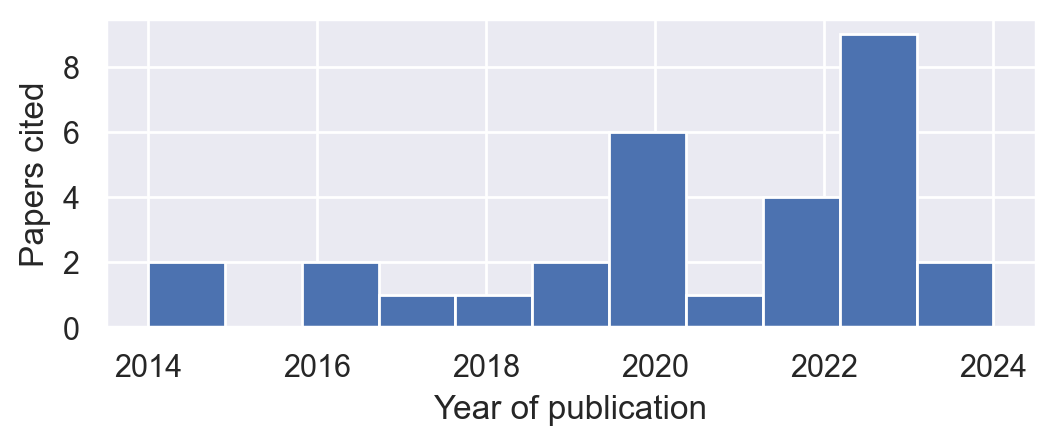
\includegraphics[height=90pt]{years_reference.png}
	\caption{Year of publication of papers cited in this thesis. These topics are novel!}
\end{figure}

One of the main strengths of my work in this thesis was having built a solid experimentation infrastructure early on, which allowed me to iterate quickly on experiments and ideas.
The program to build, run, and analyse the counterparametric-enhanced queries (which is present in \cref{appendixD} and in this project's repository) is one of the strong points of this project, and I'm sure it will be a valuable tool for future research projects.

Despite settling on the final thesis idea early, this thesis suffered from lacking a clear and well-defined research question, which emerged late in the process.
I consider this delay to have been one of the main sources of inefficiencies, since it lead to executing long experiments that contributed little to the final thesis.
One of my main takeaways from this research is the necessity to align on a well-defined research question early.

This thesis taught me how to adapt to the rapidly-changing research landscape of sequence analysis and artificial intelligence.
A lot of the methods used in this work are taken directly from previous academic papers, and this allowed me to test my hypothesis quickly while keeping a deep understanding of the context I am working on.

Most of all, I'm happy to have learned a lot about the areas of large language models and  to have been able to collaborate a bit in this very new area of research.
I plan to continue this work in the future, and I'm looking forward to contributing to the research on this area!

\subsection{Future Work}

\subsubsection{Better Categorisation of the Answers}
\label{other_problems}

To test whether two answers are equal and to know whether an answer came from parametric or contextual knowledge, the code in this thesis checks for string equality among after removing a few stop simple words such as `the'.

This solution might not be enough, and some answers classified as \Other{} should have been classifier as something else.
\Cref{bad_others} provides some examples of answers where this is the case.

\begin{table}[ht]
	\centering
	\scriptsize
	\begin{tabular}{>{\ttfamily}l@{\hspace{20pt}}>{\ttfamily}c@{\hspace{1pt}}>{\ttfamily}c@{\hspace{1pt}}c@{\hspace{1pt}}c}
		\toprule
			\bfseries \rmfamily Query & \bfseries \rmfamily Parametric Answer & \bfseries \rmfamily Query Answer & \bfseries Comparison & \bfseries Expected \\
		\midrule
			\parbox[c][100pt][t]{120pt}{[Context: The primary leader associated with The Construction of Hadrian's Wall was Napoleon Bonaparte] \\ Q: Who was the primary leader associated with The Construction of Hadrian's Wall? \\ A: The primary leader associated with The Construction of Hadrian's Wall was} &
			Emperor Hadrian &
			\parbox{75pt}{\centering Hadrian, \\ the Roman Emperor} &
			\bfseries \textcolor{MidnightBlue}{Other} &
			\bfseries \textcolor{ForestGreen}{Parametric} \\
			\parbox[c][85pt][b]{120pt}{[Context: Che Guevara was born in Kensington, London, England] \\ Q: In what city was Che Guevara born? \\ A: Che Guevara was born in \\} &
			Rosario, Argentina &
			London &
			\bfseries \textcolor{MidnightBlue}{Other} &
			\bfseries \textcolor{Maroon}{Contextual} \\
		\bottomrule
	\end{tabular}
	\caption{Example of incorrectly-categorised answers. These were categorised as "\Other{}", since their answer strings are different from both parametric and contextual answers. However, a closer look reveals that this is just either answer with a slight formatting difference.}
	\label{bad_others}
\end{table}

A more complete solution might include using another LLM to compare whether two answers are truly equal.

\subsubsection{Knowledge Grounding in Retrieval-Augmented LMs}

This thesis was originally based on a preprint, ``Knowledge Grounding in Retrieval-Augmented LMs: An Empirical Study'' \citep{knowledge_grounding_retrieval_augmented}, and contains work towards understanding how large language models retrieve data which can ultimately help prevent hallucinations.

We plan to continue this work and complete the paper created by the preprint by running the methods outlined on this thesis on retrieval-augmented LMs such as \textsc{Atlas} \citep{atlas_foundational} and \textsc{Retro} \citep{retro} and creating a full evaluation framework that specifically focuses on their grounding.
A well-grounded model should demonstrate the capability to adapt its generation based on the provided context, specially in cases like the ones experimented in this thesis when the context contradicts the model's parametric memorisation.

\subsubsection{Further Memory Locator Prediction}

The results of \cref{results_perplexity_score} show a clear difference in perplexity value between answers that come from the parametric memory of a model and those that come from a context.

This could be used to create a predictor where, given a certain answered query, it could give you a probability of the source the model used for this answer by using the perplexity of the answer and comparing against the distribution of perplexities for this model on similar questions.

In RAG-enhanced models, where the RAG context might contradict the parametric knowledge of a model, this might prevent hallucinations.

\subsubsection{Fine-tuning a LLM for a RAG Context}

Existing retrieval-augmented LMs, such as \textsc{Atlas} and \textsc{Retro}, are trained on existing models along with an index.
In the fast-moving world of large language models, this might not be ideal: the generator part of models is based on T5, a model created in 2019.
Meanwhile, between the time I started writing this thesis and this moment Meta launched a new Llama model.

The current dataset and experiments might be useful for being able to fine-tune a modern model to prefer the context generated by RAG when it contradicts its parametric knowledge.
This might improve retrieval-augmented models, and make it easier to use them with newer models.


% \appendix{}

% \section{All Questions Used as Knowledge}


\bibliography{knowledge_grounding.bib}

\end{document}
